\documentclass[11pt]{article}

\usepackage{graphicx}
\usepackage{glossary}
\usepackage{url}
\usepackage{xspace}
\usepackage{bold-extra}
\usepackage{listings}
\usepackage[final]{pdfpages}

\graphicspath{{figures/}}


\newcommand{\JUnit}{\textsc{JUnit}\xspace}
\newcommand{\JExample}{\textsc{JExample}\xspace}

\newcommand{\ttt}[1]{\texttt{#1}}

\newcommand{\nb}[2]{
    \fbox{\bfseries\sffamily\scriptsize#1: #2}
    }

\newcommand{\todo}[1]{\nb{TODO}{#1}}

\newcommand{\setup}{\ttt{setup()}}
\newcommand{\testPush}{\ttt{testPush()}}
\newcommand{\testPushAll}{\ttt{testPushAll()}}
\newcommand{\testPop}{\ttt{testPop()}}
\newcommand{\testPopFails}{\ttt{testPopFails()}}

%%%%%%%%%%%%%%%%%%%%%%%%%%%%%%%%%%%%%%%%%%%%%%%%%%%%%%%%%%%%
\begin{document}

\title{JExample}

\author{Lea H\"ansenberger\\
	Supervised by: Adrian Kuhn\\
	University of Bern, Switzerland\\
	Software Composition Group
}

\maketitle

\begin{abstract}

\end{abstract}

%%%%%%%%%%%%%%%%%%%%%%%%%%%%%%%%%%%%%%%%%%%%%%%%%%%%%%%%%%%%
\section{Introduction}

\todo{why software testing}\\\\
\todo{what we gain from JUnit}\\\\
\todo{why dependencies}\\\\
 
\section{Related Work}

\section{Example}

In this section I will illustrate the difference between composed and conventional test methods by exercising a sample test case. Unit under test is a simple Stack implementation. A convention test case would go as follows:

\begin{lstlisting}[label=lst:junit,caption=Conventional \JUnit test case.]
public class StackTest {

    private Stack stack;

    @Before
    public void setup() {
        stack = new Stack();
    }

    @Test
    public void testPush() {
        stack.push("Foo");
        assertFalse(stack.isEmpty());
        assertEquals("Foo", stack.top());
    }

    @Test
    public void testPop() {
        stack.push("Foo");
        Object top = stack.pop();
        assertTrue(stack.isEmpty());
        assertEquals("Foo", top);
    }

    @Test(expected=IllegaleStateException.class)
    public void testPopFails() {
        stack.pop();
    }

    @Test
    public void testPushAll() {
        List list = Arrays.asList(new String[] { ... });
        last = list.get(list.size() - 1);
        stack.pushAll(list);
        assertEquals(last, stack.top());
    }

}
\end{lstlisting}

When running Listing \ref{lst:junit} \setup is executed before every test method and the test fixture is passed as class attribute. We could say, that all the test methods depend on \setup. In \JExample \setup would be a normal test method returning an instance of a Stack.

\begin{lstlisting}[label=lst:setup,caption=Promote fixture to test with return value.]
    @Test
    public Stack setup() {
        Stack empty = new Stack();
        assertTrue(empty.isEmpty());
        assertEquals(null, empty.top()));
        return empty;
    }
\end{lstlisting}

Please note, that by setting up the fixture in a test method instead of a setup method, the initialization of the fixture can be tested, too.
\testPush and \testPopFails need to define \setup as their dependency because they need an empty stack. This is done by annotating them with \ttt{@Depends}. Furthermore, they need to take a Stack as an argument.

\begin{lstlisting}[label=lst:testpush,caption=Take another test's result as input value.]
    @Test
    @Depends("setup")
    public Stack testPush(Stack stack) {
        stack.push("Foo");
        assertFalse(empty.isEmpty());
        assert("Foo", empty.top());
        return stack;
    }

    @Test(expected= IllegalStateException.class)
    @Depends("setup")
    public Stack testPopFails(Stack empty) {
        stack.pop();
    }
\end{lstlisting}

When running Listing \ref{lst:testPush} \JExample runs first \setup, as it is the root of the dependency hierarchy. If \setup run successfully \testPush and \testPopFails are run with the return value from \setup as argument (if \setup fails, \testPush and \testPopFails are ignored).
In order to have the same state of the stack for both the dependents the return value needs to be cloned. Of course this can only be accomplished if the return value's class or one of its superclasses implements \verb|Object.clone()|.
Let's now reconsider Listing \ref{lst:junit} to find deeper levels of dependencies in order to get a real graph of composed test methods.
Indeed, we find two methods that depend on \testPush: \testPop cannot be executed without pushing an element on the stack first and \testPushAll will probably also fail if pushing a single element fails.

The new implementation of \testPop needs to depend on \testPush's return value. This also avoids the duplicate call to \ttt{push}.

\begin{lstlisting}[label=lst:testpop,caption=Avoid code duplication using dependencies.]
    @Test
    @Depends("testPush")
    public Stack testPop(Stack stack) {
        Object top = stack.pop();
        assertEquals(true, empty.isEmpty());
        assertEquals("Foo", top);
        return stack;
    }
\end{lstlisting}

\testPushAll needs a list of elements as a second argument. Let's assume we have a class \ttt{ListTest} with a method \ttt{testAddAll()}. The refactored \testPushAll looks as follows. Note that a test may have more than one dependency that can also refer to methods in other test case files.

\begin{lstlisting}[label=lst:testpushall,caption=A test may have multiple dependencies.]
    @Test
    @Depends("testPush;ListTest.testAddAll")
    public stack testPushAll(Stack stack, List list) {
        stack.pushAll(list);
        last = list.get(list.size() - 1);
        assertEquals(last, stack.top());
        return stack;
    }
\end{lstlisting}

With \ttt{Stack}'s \ttt{push} method failing, the test result would be two green, one red and two white tests (see Figure \ref{fig:testPush}).

\begin{figure}[htbp]
 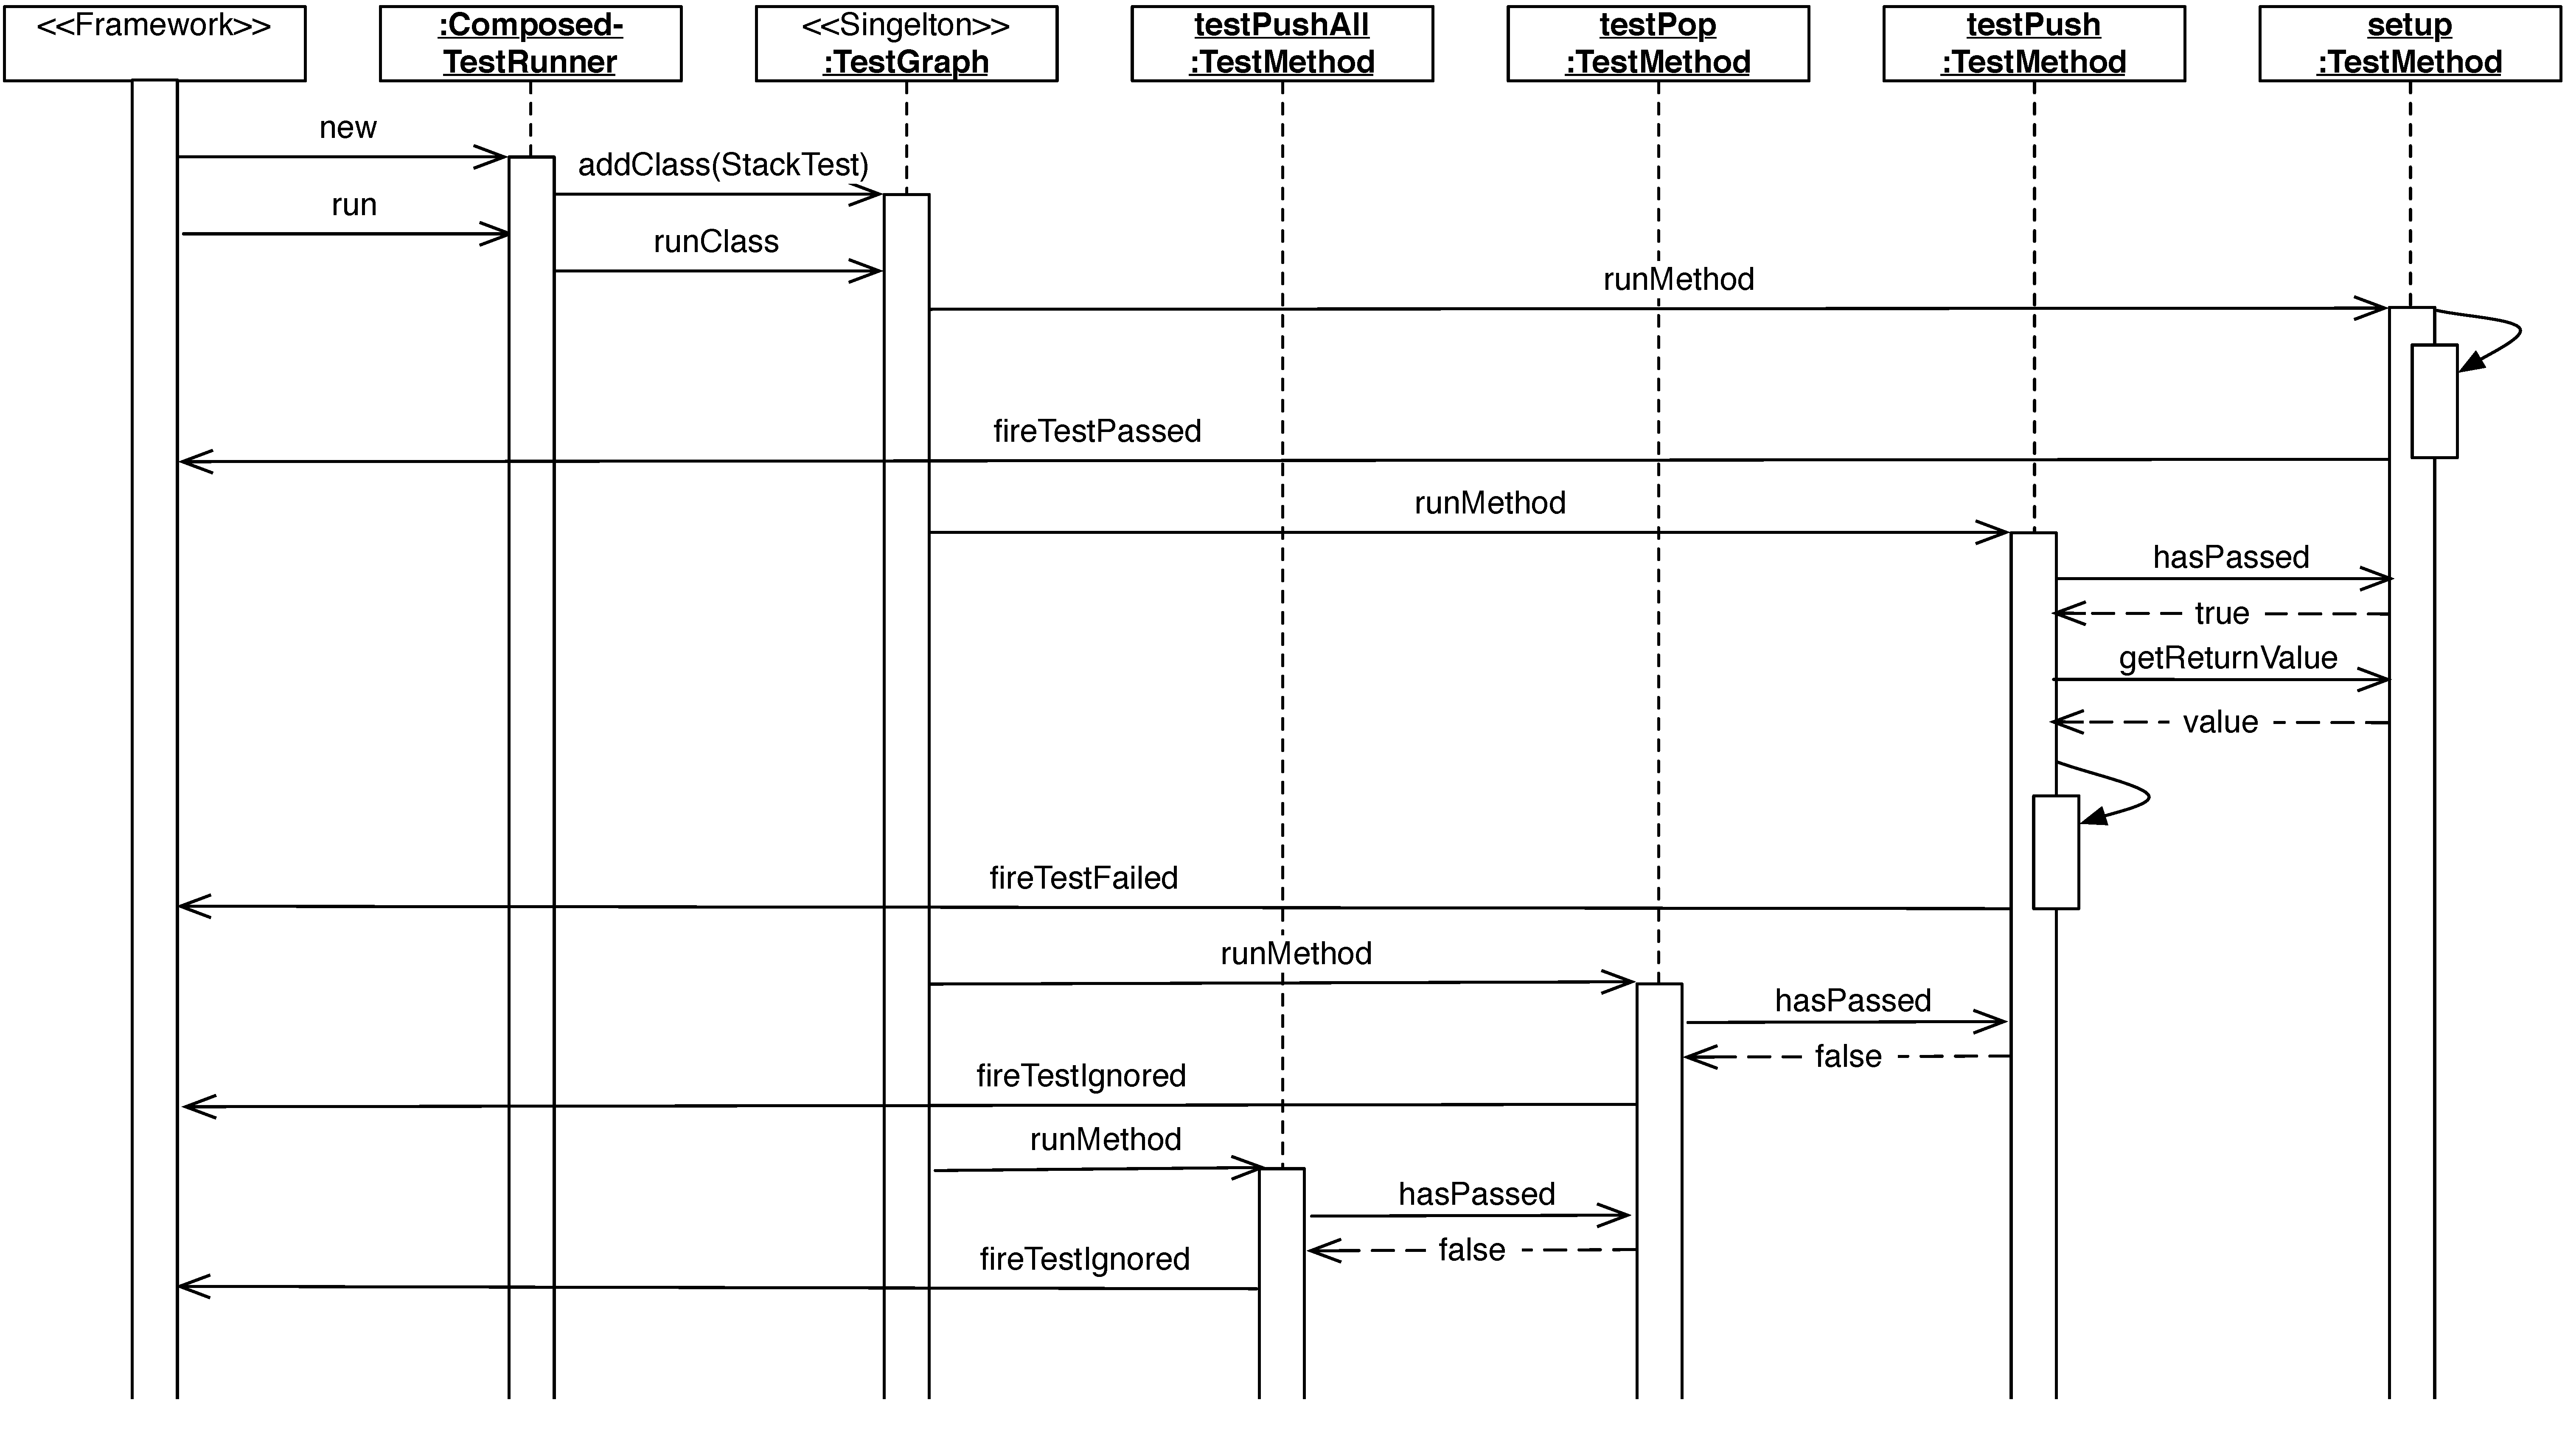
\includegraphics[width=15.0cm]{testPush.pdf}
 \caption{}
 \label{fig:testPush}
\end{figure}

\section{Implementation}

To extend the \JUnit Framework mainly one class is needed. The Runner. This class consists of three parts corresponding to the three steps of a test run.

\begin{enumerate}
 \item a constructor for the initialization of the Runner
 \item a method \verb|Runner.run()| to run the test methods
 \item a method \verb|Runner.getDescription()| to get information about the run
\end{enumerate}
In \JExample \verb|ComposedTestRunner| is only a delegator. It passes the responsibilities to the \verb|TestGraph|. The reason will be explained later on.\\
See Figure \ref{fig:classDiag} for the important classes of \JExample.

\begin{figure}[htbp]
 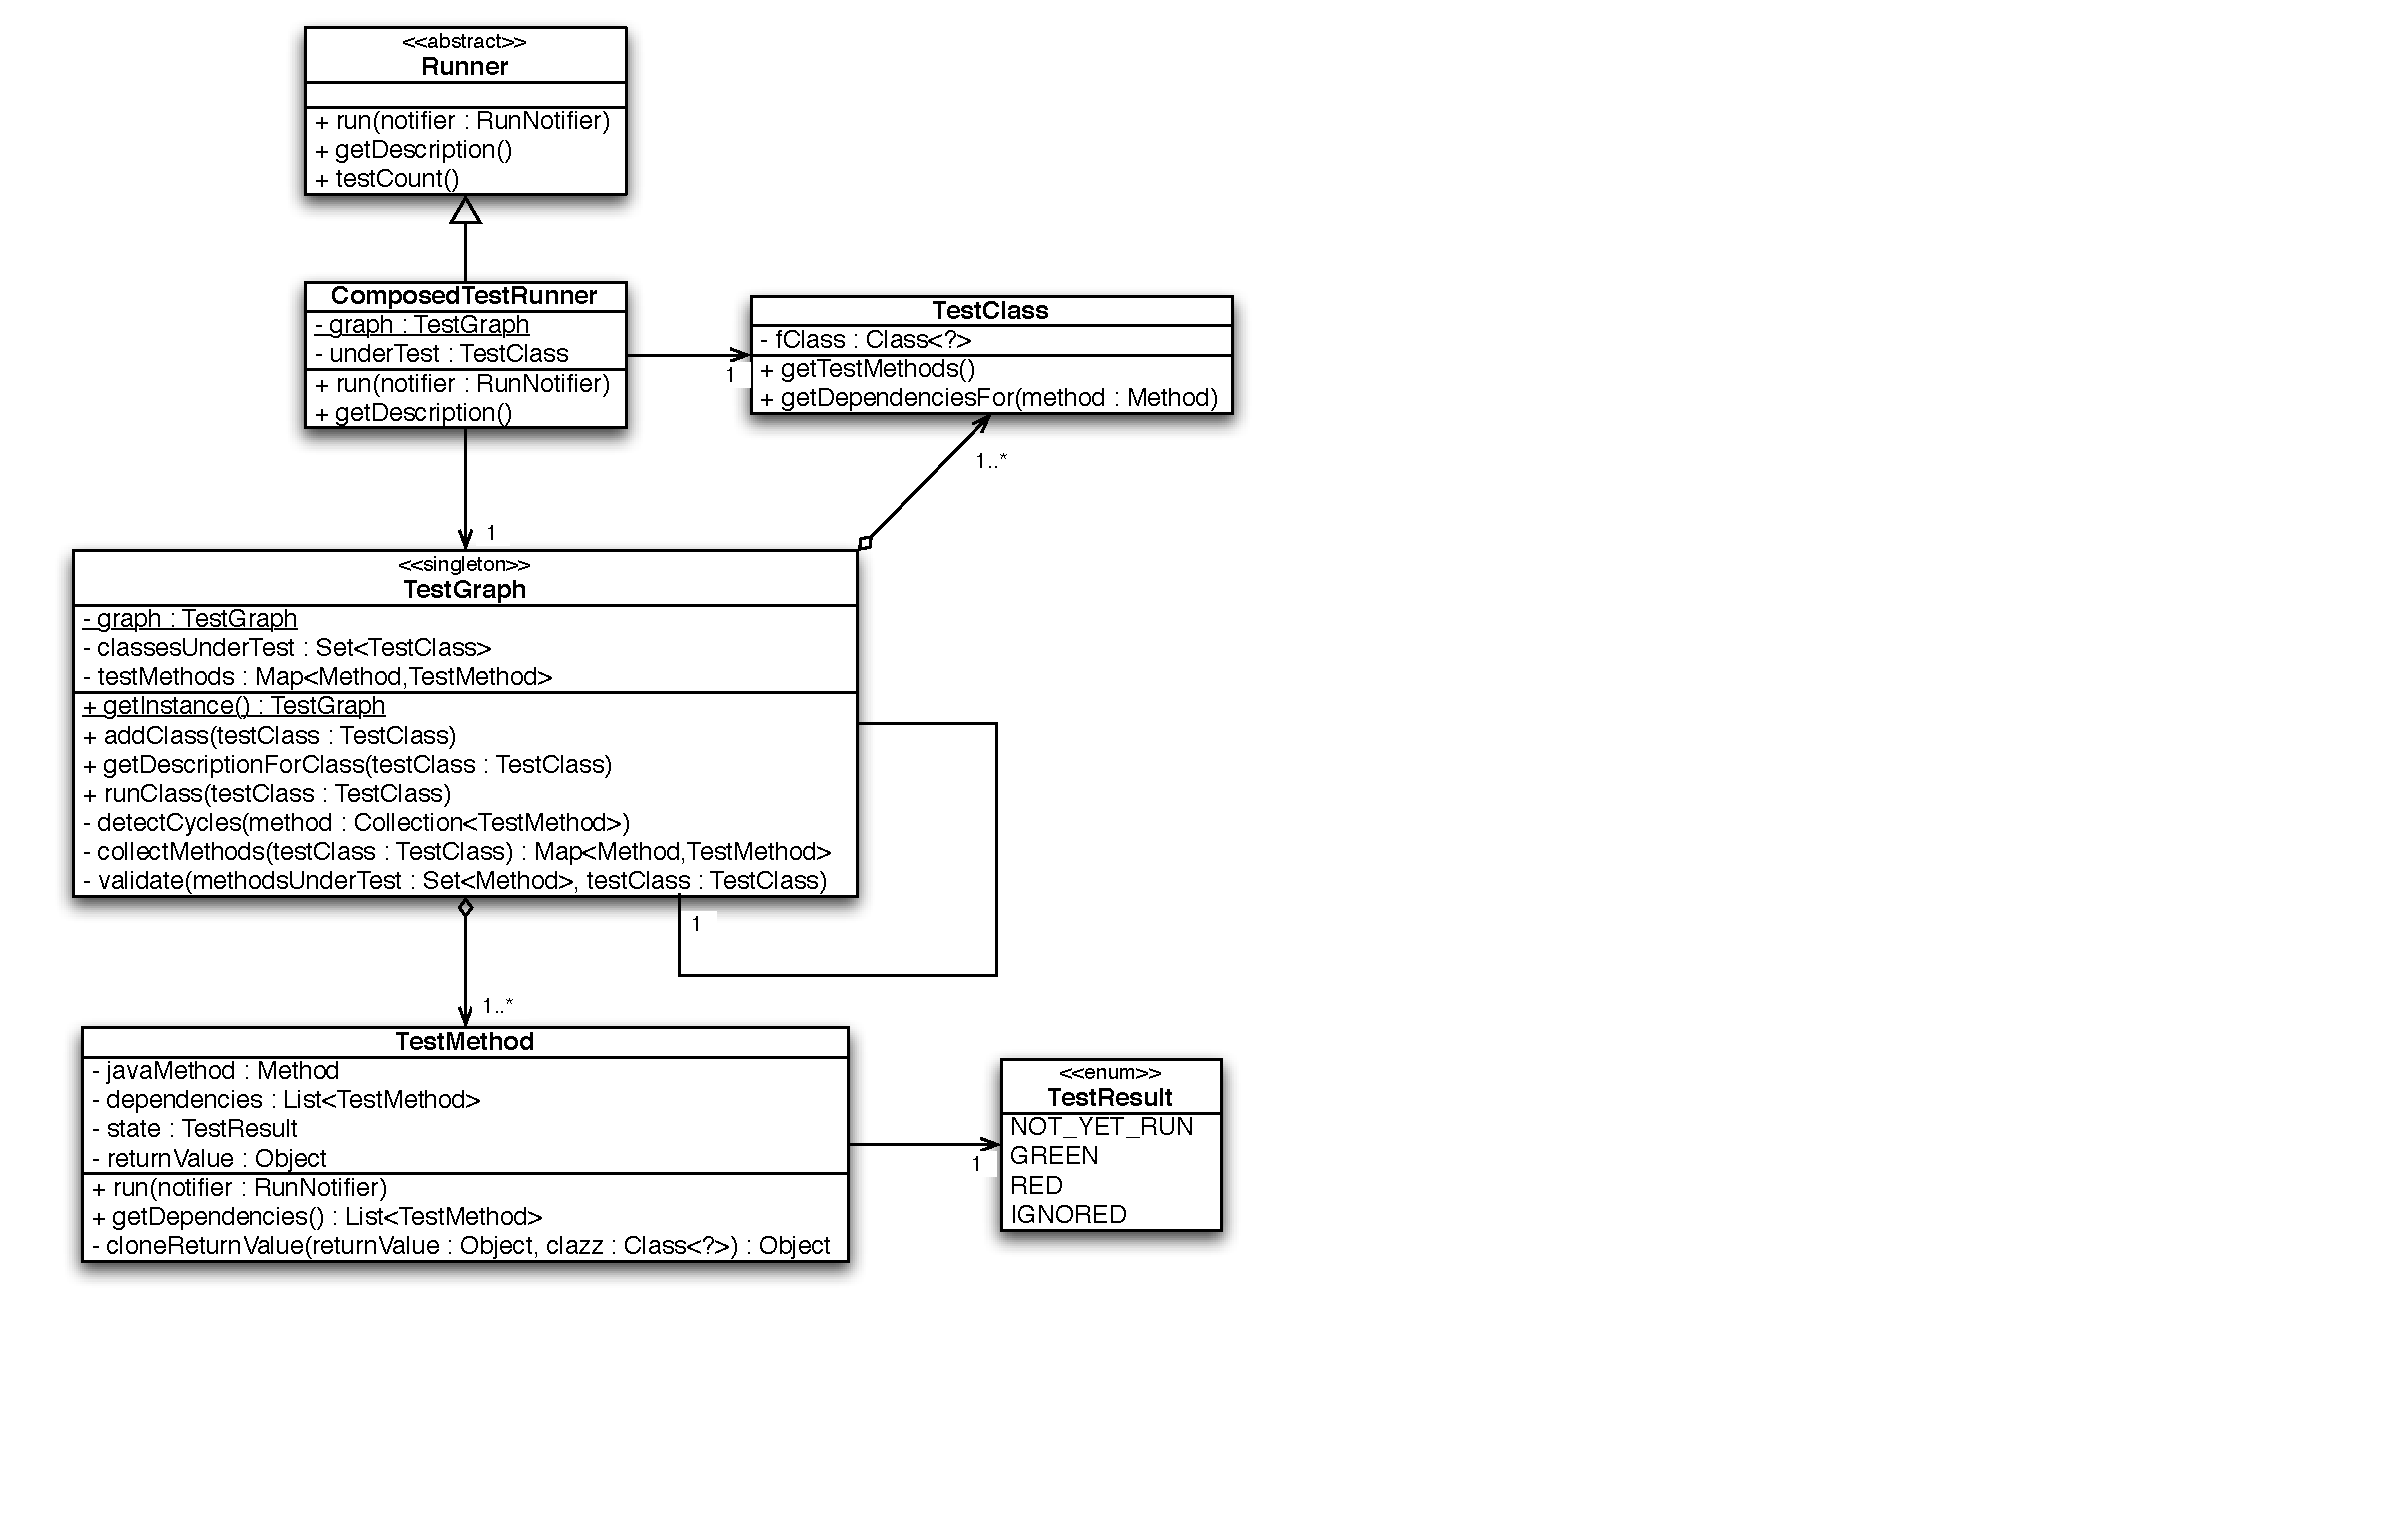
\includegraphics[width=24.0cm]{classdiagram.pdf}
 \caption{Class Diagram}
 \label{fig:classDiag}
\end{figure}

For \JExample also wrapper classes and validators needed to be adapted. \JUnit only allows methods without parameters and with return type void. As methods in \JExample need to be allowed to take arguments and return objects, the validation of the methods needed to be adapted. See Figure \ref{fig:classDiagInit} for the classes responsible for the initialization and validation of a test run.

\begin{figure}[htbp]
 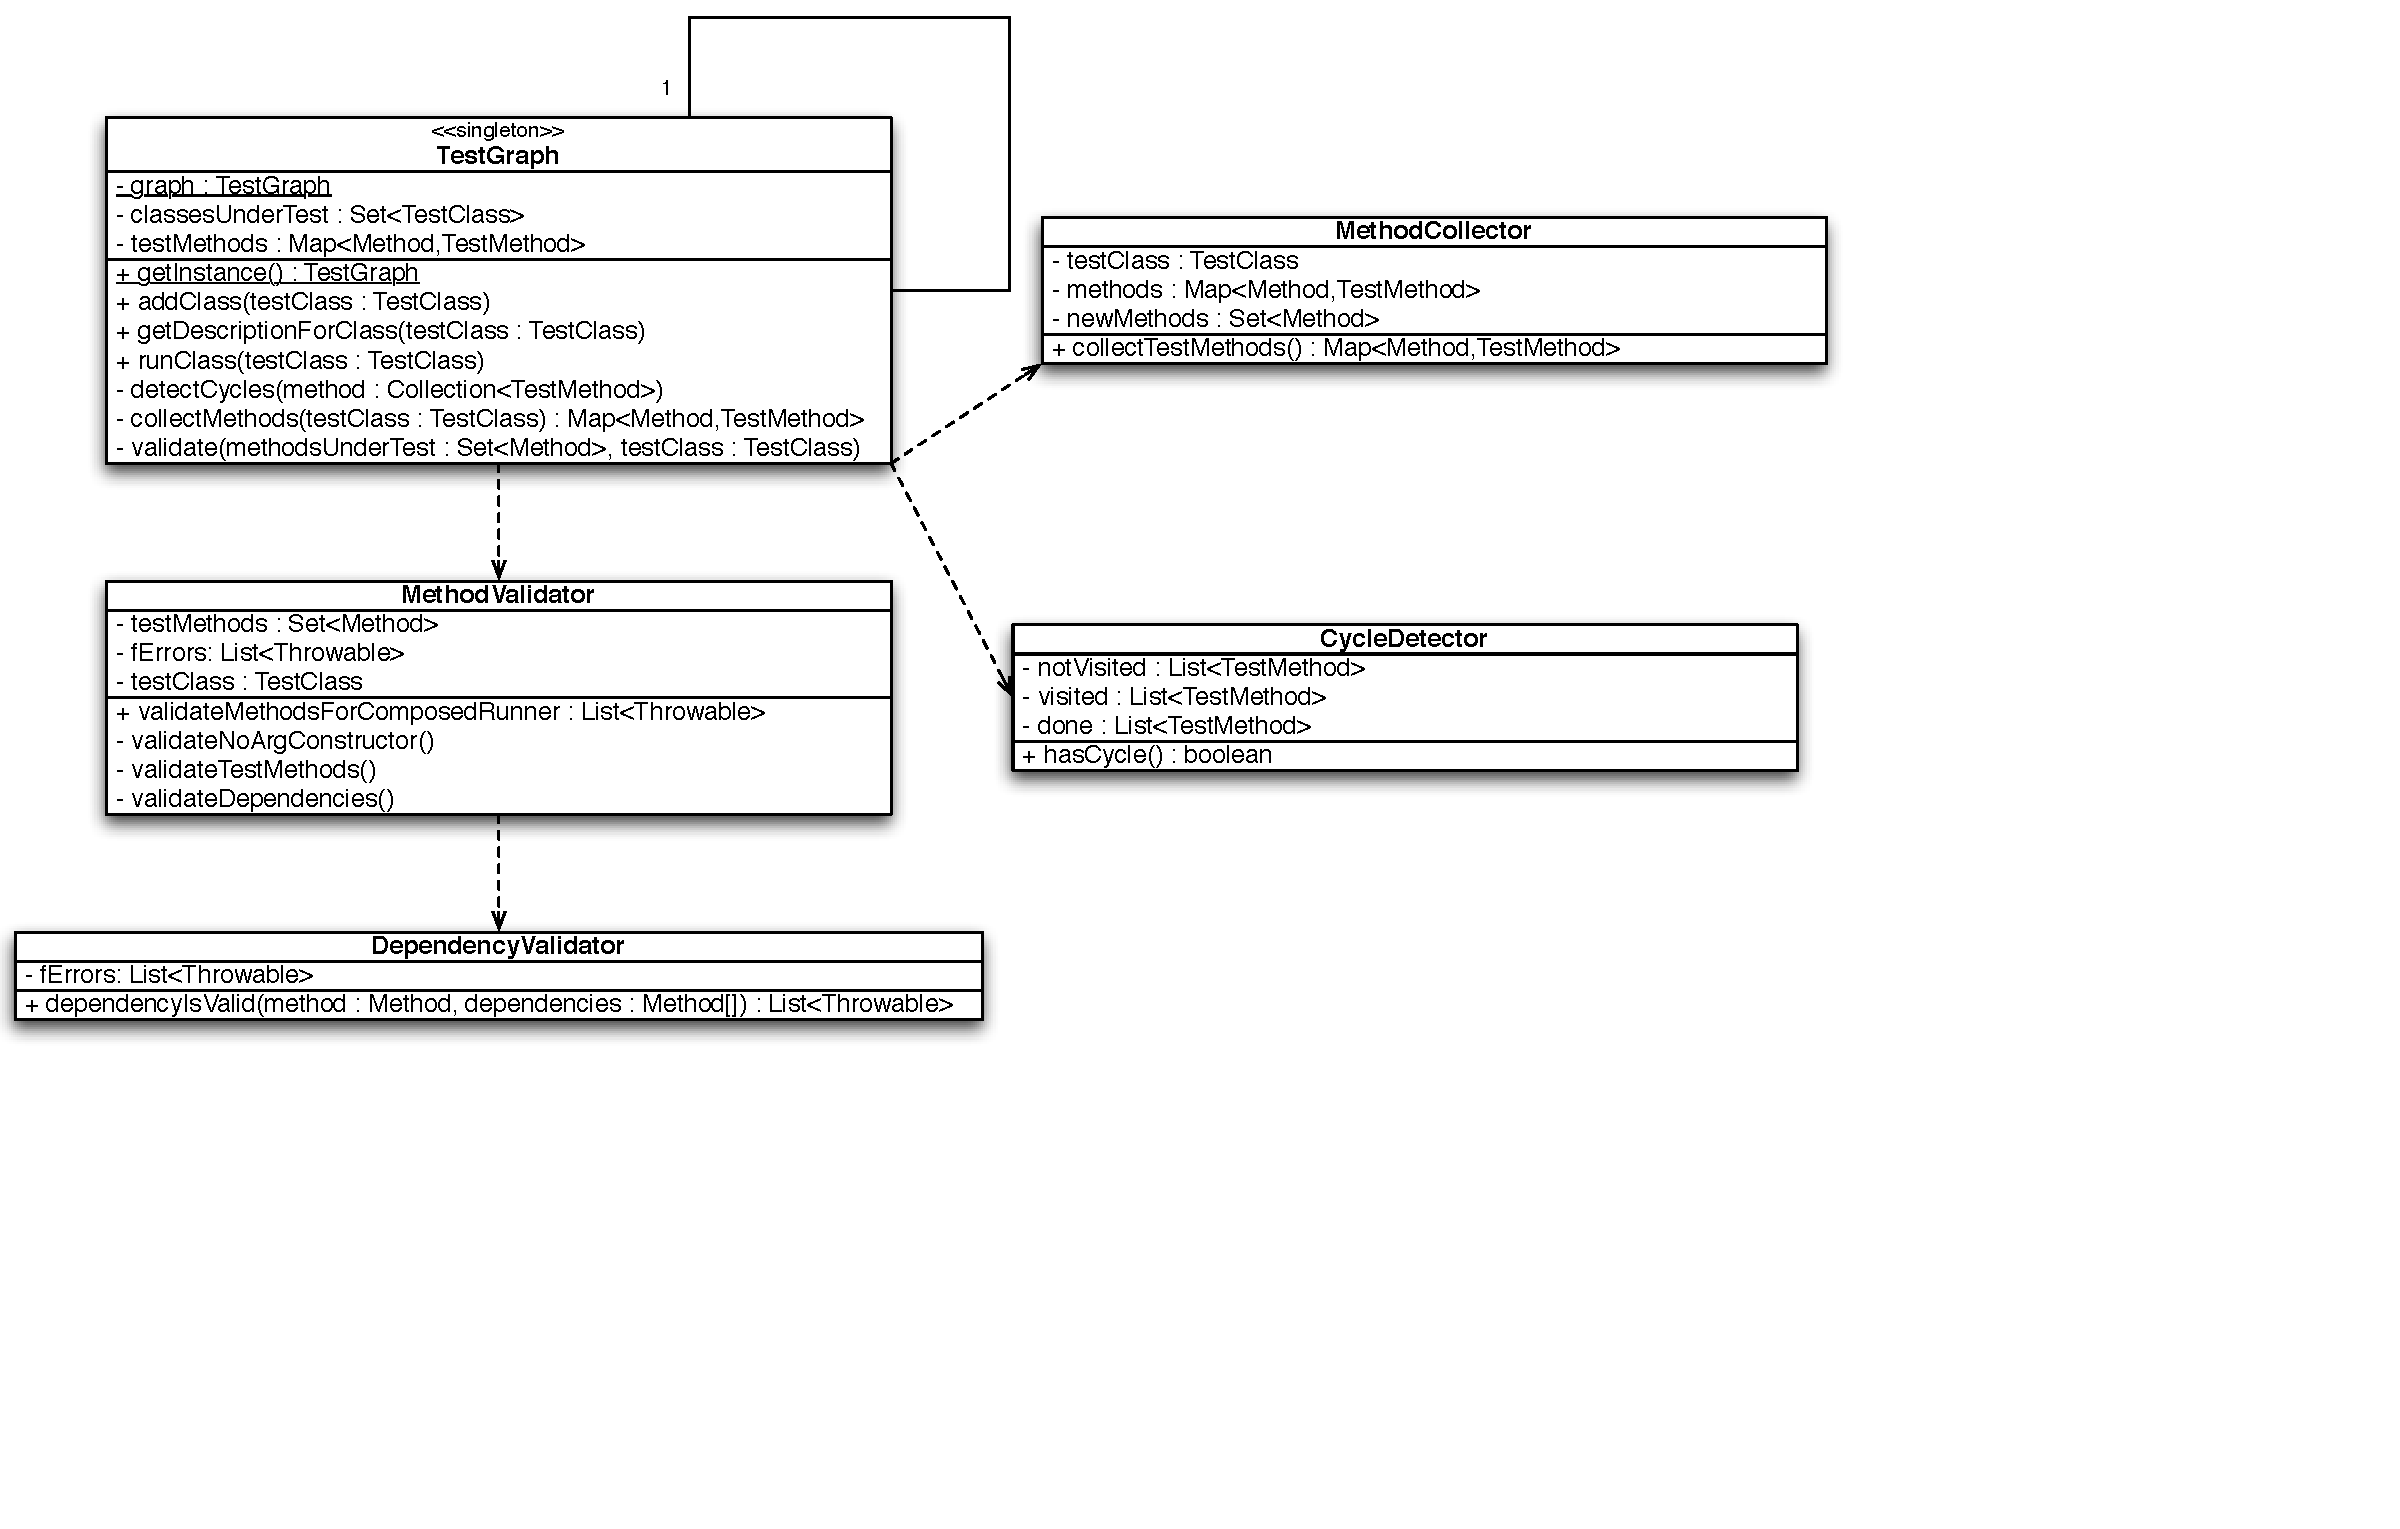
\includegraphics[width=20.0cm]{classdiagramInit.pdf}
 \caption{Initialization Test Run}
 \label{fig:classDiagInit}
\end{figure}

In \JUnit a separate class is responsible for running the test methods. In \JExample \verb|TestMethod| is responsible for running its wrapped method. A \verb|TestMethod| knows its dependencies and its return value. Therefore it can simply ask its dependencies if they passed and get possible return values.

In the following section I will go into more detail for the single, most important classes of \JExample

\subsubsection{The ComposedTestRunner}

The Runner is the main connection to the \JUnit Framework. It extends the abstract class \verb|org.junit.runner.Runner| and implements two methods \verb|Runner.run()| and \verb|Runner.getDescription()|. A test run consists of three steps:
\begin{enumerate}
 \item initializing the Runner, this includes collecting and validating methods and test dependencies
 \item running the methods
 \item getting the description of the run
\end{enumerate}

\subsubsection{The TestGraph}

The real Runner in \JExample is the \verb|TestGraph|. The reason for delegating this responsibility to another class is that we wanted the Runner to be a singleton. A singleton is necessary because a method can depend on a method from another class. When running a test suite, this makes sure that every method is collected and run only once. Therefore, every method is counted only once and the run count correpsonds to the number of methods. This is possible because of the behaviour of \JUnit when running multiple classes at once. First, a Runner per class is initialized, then all the classes are run and in the end, the description for every class is collected.

\todo{ev. insert sequence diagram for the three steps of a test run with two or more classes}

The \verb|TestGraph| reflects the three steps of a test run in its three public methods \verb|addClass()| for the initialization, \verb|runClass()| for running the methods and \verb|getDescriptionForClass()| for getting the description of all the run methods. If methods declare dependencies to methods of other classes, those dependencies are added and run as they were part of the class under test. When getting the description, however, it is made clear which method belongs to which class.

\subsubsection{The TestClass}

\verb|TestClass| is a wrapper for the class under test. It returns all the test methods by filtering those who are annotated with \verb|@Test|. In addition it gets the list of dependencies for methods annotated with \verb|@Depends| by getting the methods represented by the String value of the annotation.

\subsubsection{The TestMethod}

\verb|TestMethod| is the wrapper for the methods to be run. The \verb|TestMethod| knows its dependencies, its \verb|TestResult| and its return value after it was run. Possible test results are

\begin{description}
 \item[NOT\_YET\_RUN] the method has not been run yet
 \item[GREEN] the method was run and finished successfully
 \item[RED] the method was run but failed
 \item[IGNORED] the method is either annotated with \verb|@Ignore| or one of its dependencies has the result RED or IGNORED
 \end{description}

It makes sure, that all of its dependencies have been run before it's run itself. It also checks the results of its dependencies. If one of the dependencies failed or was ignored, either because of the annotation \verb|@Ignore| or because one of its dependencies failed or was ignored, it informs the \verb|RunNotifier| that it is ignored, too.

If a method takes arguments \verb|TestMethod| gets the return values from the dependencies and passes them to the method to be run. The return value is cloned before it is passed to the method if its class or one of its superclasses implements \verb|Cloneable| and overrides \verb|Object.clone()|.

\section{Lesson learned}

\begin{appendix}
\section{Javadoc}
\todo{modify docs.tex to good format}
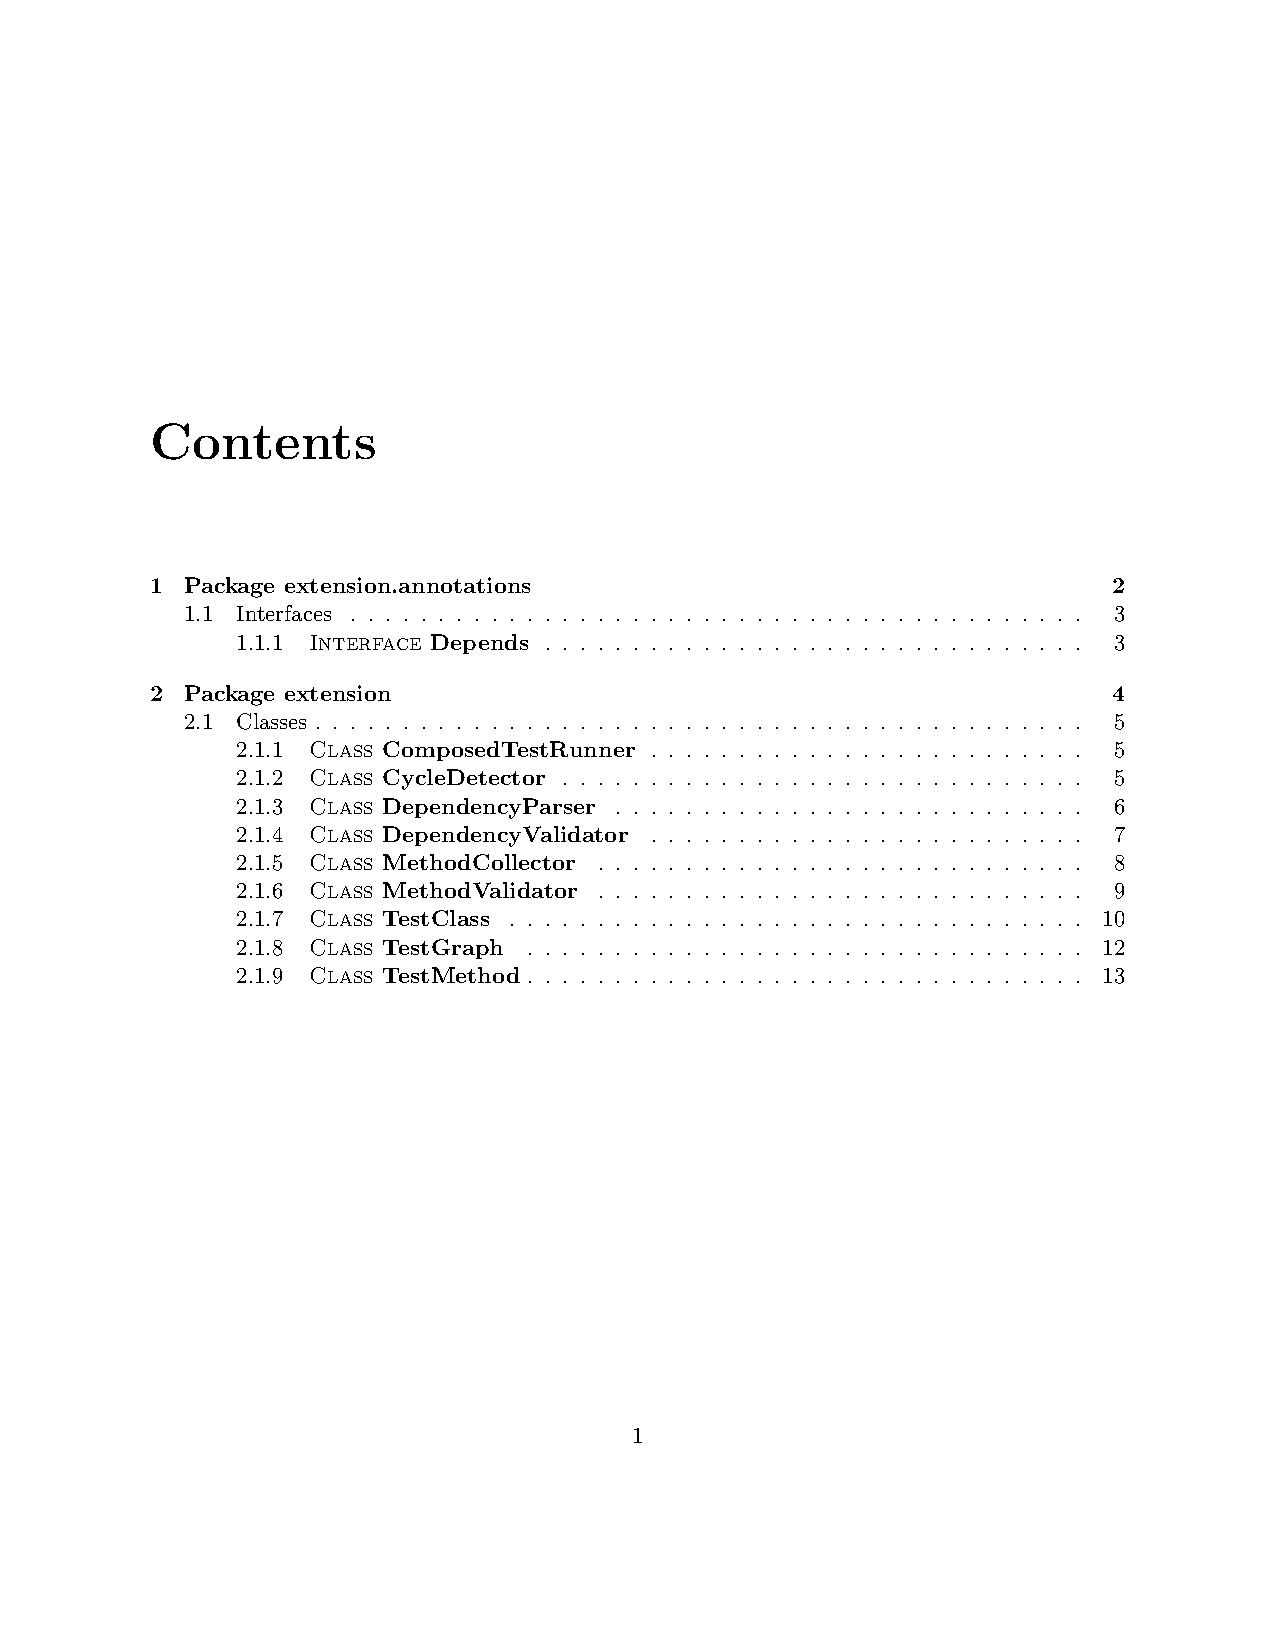
\includepdf[pages=1-13]{figures/docs.pdf}

\section{Ullman Original}
\lstinputlisting[label=lst:ullmanorig,caption=TestUllman.java]{tests/TestUllman.java}

\section{Ullman refactored}
\lstinputlisting[label=lst:ullmancomp,caption=IsomorphTestUllman.java]{tests/IsomorphTestUllman.java}
\lstinputlisting[label=lst:ullmancomp,caption= SimpleSubgraphTest.java]{tests/SimpleSubgraphTest.java}
\lstinputlisting[label=lst:ullmancomp,caption= SpecialSubgraphTest.java]{tests/SpecialSubgraphTest.java}
\lstinputlisting[label=lst:ullmancomp,caption= VertexPairTest.java]{tests/VertexPairTest.java}

\end{appendix}

\end{document}

